\section{Task: Associate Target Reports}
\label{sec:task_associate_tr} 

This task allows creation of UTNs and target report association based on Mode S Addresses.

Please note that if no Mode S information exists in the database, or usage of UTNs is not needed, these step does not have to be performed. \\

If usage the evaluation feature is wanted, running this task is required.

\begin{figure}[H]
  \hspace*{-2.5cm}
    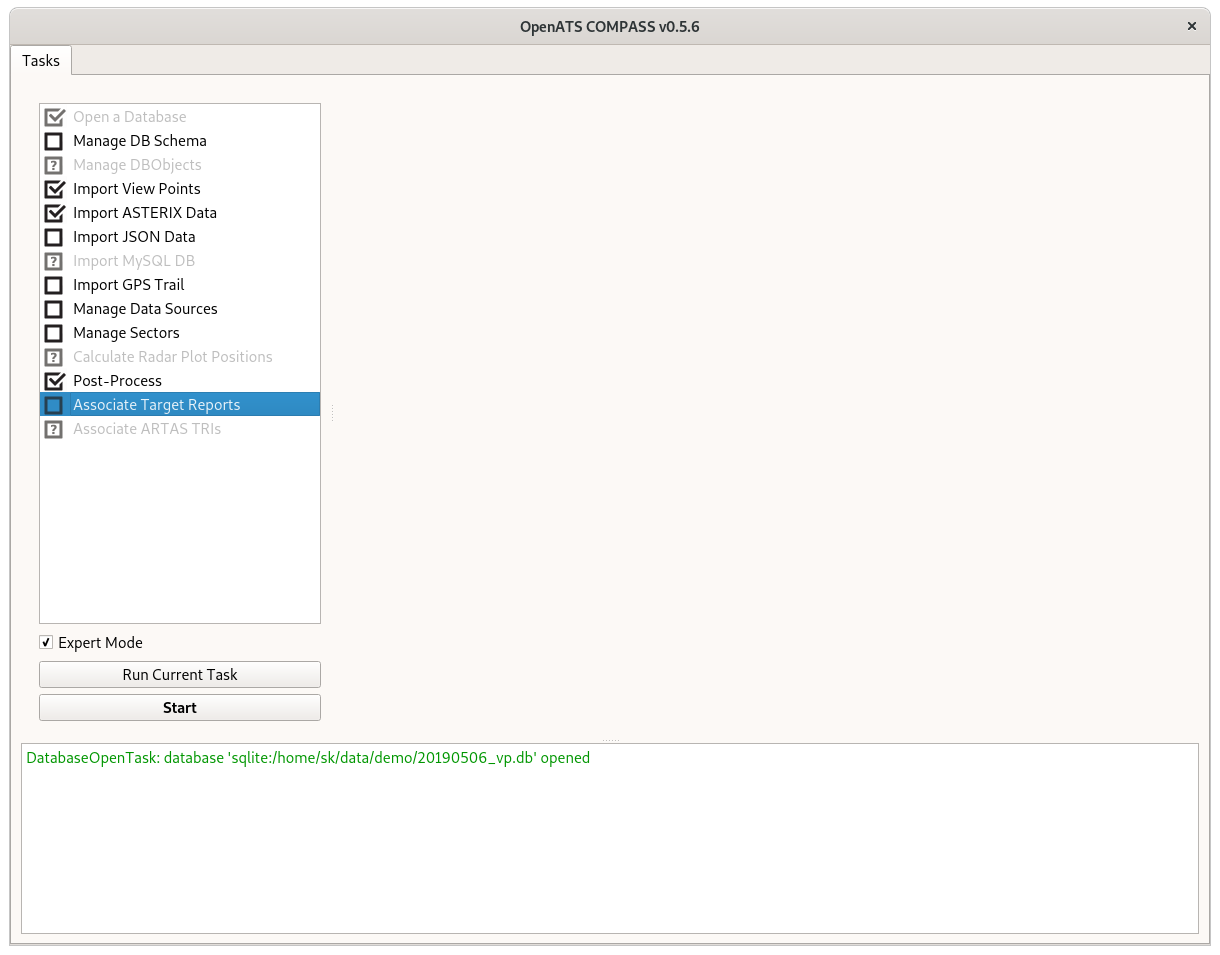
\includegraphics[width=19cm]{../screenshots/tr_association_config.png}
  \caption{Task: Associate Target Reports}
\end{figure}

Currently this task has no configuration needing to be set. \\

The UTNs are created by simply associating all target reports (from all DBObjects) by their Mode S address. Each found unique Mode S target address is assigned a unique UTN, to which in turn all target reports with this address are associated. \\

Target reports without a Mode S address are not associated to any UTN. \\

The author is aware that this does not allow a lot of meaningful use cases, so this task will be improved in the near future to include association based on local track numbers, Mode A/C codes and position metrics. \\

To run the task, click the 'Run Current Task' button. After the assocations are saved, the task is done:

\begin{figure}[H]
  \center
    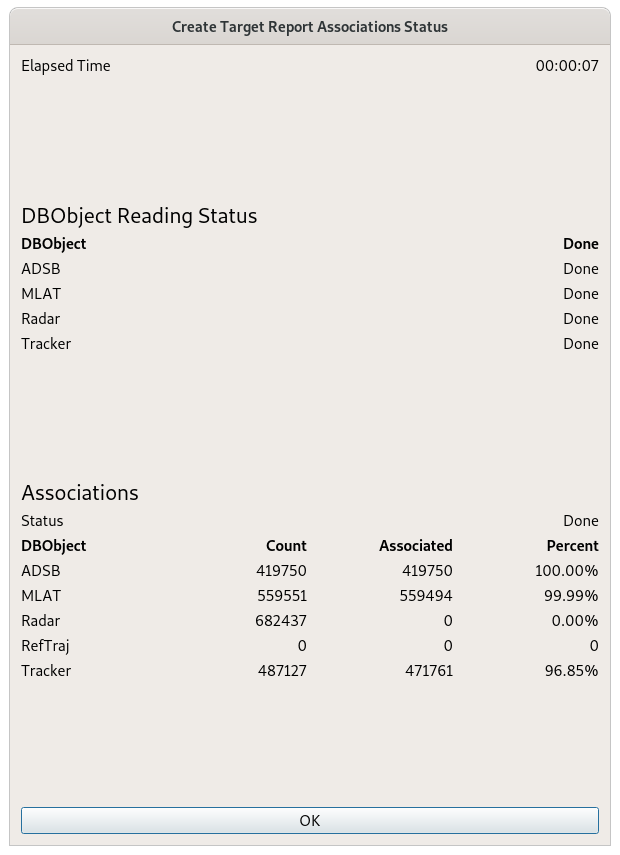
\includegraphics[width=11cm]{../screenshots/tr_association_done.png}
\end{figure}
